\documentclass[10pt,mathserif]{beamer}

\usepackage{graphicx,amsmath,amssymb,tikz,psfrag}
\usepackage{pythonhighlight, xcolor}

% ------------------------------------------------------------------------
% Packages
% ------------------------------------------------------------------------
\usepackage{amsmath}
\usepackage{tabularx}

% ------------------------------------------------------------------------
% Macros
% ------------------------------------------------------------------------
%~~~~~~~~~~~~~~~
% List shorthand
%~~~~~~~~~~~~~~~
\newcommand{\BIT}{\begin{itemize}}
\newcommand{\EIT}{\end{itemize}}
\newcommand{\BNUM}{\begin{enumerate}}
\newcommand{\ENUM}{\end{enumerate}}
%~~~~~~~~~~~~~~~
% Text with quads around it
%~~~~~~~~~~~~~~~
\newcommand{\qtext}[1]{\quad\text{#1}\quad}
%~~~~~~~~~~~~~~~
% Shorthand for math formatting
%~~~~~~~~~~~~~~~
\newcommand\mbb[1]{\mathbb{#1}}
\newcommand\mbf[1]{\mathbf{#1}}
\def\mc#1{\mathcal{#1}}
\def\mrm#1{\mathrm{#1}}
%~~~~~~~~~~~~~~~
% Common sets
%~~~~~~~~~~~~~~~
\def\reals{\mathbb{R}} % Real number symbol
\def\integers{\mathbb{Z}} % Integer symbol
\def\rationals{\mathbb{Q}} % Rational numbers
\def\naturals{\mathbb{N}} % Natural numbers
\def\complex{\mathbb{C}} % Complex numbers
\def\simplex{\mathcal{S}} % Simplex
%~~~~~~~~~~~~~~~
% Common functions
%~~~~~~~~~~~~~~~
\renewcommand{\exp}[1]{\operatorname{exp}\left(#1\right)} % Exponential
\def\indic#1{\mbb{I}\left({#1}\right)} % Indicator function
\providecommand{\maximize}{\mathop\mathrm{maximize}} % Defining math symbols
\providecommand{\minimize}{\mathop\mathrm{minimize}}
\providecommand{\argmax}{\mathop\mathrm{arg max}}
\providecommand{\argmin}{\mathop\mathrm{arg min}}
\providecommand{\arccos}{\mathop\mathrm{arccos}}
\providecommand{\asinh}{\mathop\mathrm{asinh}}
\providecommand{\dom}{\mathop\mathrm{dom}} % Domain
\providecommand{\range}{\mathop\mathrm{range}} % Range
\providecommand{\diag}{\mathop\mathrm{diag}}
\providecommand{\tr}{\mathop\mathrm{tr}}
\providecommand{\abs}{\mathop\mathrm{abs}}
\providecommand{\card}{\mathop\mathrm{card}}
\providecommand{\sign}{\mathop\mathrm{sign}}
\def\rank#1{\mathrm{rank}({#1})}
\def\supp#1{\mathrm{supp}({#1})}
%~~~~~~~~~~~~~~~
% Common probability symbols
%~~~~~~~~~~~~~~~
\def\E{\mathbb{E}} % Expectation symbol
\def\Earg#1{\E\left[{#1}\right]}
\def\Esubarg#1#2{\E_{#1}\left[{#2}\right]}
\def\P{\mathbb{P}} % Probability symbol
\def\Parg#1{\P\left({#1}\right)}
\def\Psubarg#1#2{\P_{#1}\left[{#2}\right]}
\def\Cov{\mrm{Cov}} % Covariance symbol
\def\Corr{\mrm{Corr}} % Covariance symbol
\def\Covarg#1{\Cov\left[{#1}\right]}
\def\Covsubarg#1#2{\Cov_{#1}\left[{#2}\right]}
\def\Corrsubarg#1#2{\Corr_{#1}\left[{#2}\right]}
\def\Var{\mrm{Var}}
\def\Vararg#1{\Var\left(#1\right)}
\def\Varsubarg#1#2{\Var_{#1}\left(#2\right)}
\newcommand{\family}{\mathcal{P}} % probability family
\newcommand{\eps}{\epsilon}
\def\absarg#1{\left|#1\right|}
\def\msarg#1{\left(#1\right)^{2}}
\def\logarg#1{\log\left(#1\right)}
%~~~~~~~~~~~~~~~
% Distributions
%~~~~~~~~~~~~~~~
\def\Gsn{\mathcal{N}}
\def\Ber{\textnormal{Ber}}
\def\Bin{\textnormal{Bin}}
\def\Unif{\textnormal{Unif}}
\def\Mult{\textnormal{Mult}}
\def\Cat{\textnormal{Cat}}
\def\Gam{\textnormal{Gam}}
\def\InvGam{\textnormal{InvGam}}
\def\NegMult{\textnormal{NegMult}}
\def\Dir{\textnormal{Dir}}
\def\Lap{\textnormal{Laplace}}
\def\Bet{\textnormal{Beta}}
\def\Poi{\textnormal{Poi}}
\def\HypGeo{\textnormal{HypGeo}}
\def\GEM{\textnormal{GEM}}
\def\BP{\textnormal{BP}}
\def\DP{\textnormal{DP}}
\def\BeP{\textnormal{BeP}}
%~~~~~~~~~~~~~~~
% Theorem-like environments
%~~~~~~~~~~~~~~~

%-----------------------
% Probability sets
%-----------------------
\newcommand{\X}{\mathcal{X}}
\newcommand{\Y}{\mathcal{Y}}
\newcommand{\D}{\mathcal{D}}
\newcommand{\Scal}{\mathcal{S}}
%-----------------------
% vector notation
%-----------------------
\newcommand{\bx}{\mathbf{x}}
\newcommand{\by}{\mathbf{y}}
\newcommand{\bt}{\mathbf{t}}
\newcommand{\xbar}{\overline{x}}
\newcommand{\Xbar}{\overline{X}}
\newcommand{\tolaw}{\xrightarrow{\mathcal{L}}}
\newcommand{\toprob}{\xrightarrow{\mathbb{P}}}
\newcommand{\laweq}{\overset{\mathcal{L}}{=}}
\newcommand{\F}{\mathcal{F}}


%% formatting

\mode<presentation>
{
\usetheme{default}
}
\setbeamertemplate{navigation symbols}{}
\usecolortheme[rgb={0.13,0.28,0.59}]{structure}
\setbeamertemplate{itemize subitem}{--}
\setbeamertemplate{frametitle} {
	\begin{center}
	  {\large\bf \insertframetitle}
	\end{center}
}

\AtBeginSection[]
{
	\begin{frame}<beamer>
		\frametitle{Outline}
		\tableofcontents[currentsection,currentsubsection]
	\end{frame}
}

%% begin presentation

\title{\large \bfseries Bayesian Deep Learning}

\author{Kris Sankaran\\[3ex]
Nepal Winter School in AI}

\date{\today}

\begin{document}
\maketitle

\section{Introduction}
\label{sec:introduction}

\begin{frame}
  \frametitle{Learning Objectives}
  \begin{itemize}
  \item Trace historical development of Bayesian ML, from Variational Inference
    to Bayesian Deep Learning
  \item Add some more models and algorithm to personal catalog of examples
  \item Understand underlying math and code for example algorithms
  \end{itemize}
\end{frame}

\begin{frame}
  \frametitle{Papers from 1990}
  \begin{itemize}
  \item Gelfand and Smith: Renaissance in Bayesian Inference
  \item LeCun et. al.: Early proof of representation learning through neural networks
  \item Common: Use computation to automate tediour, expert-labor intensive processes
  \item Tension: The ``two cultures''... prediction or inference?
  \end{itemize}
  \begin{figure}
    \subfigure{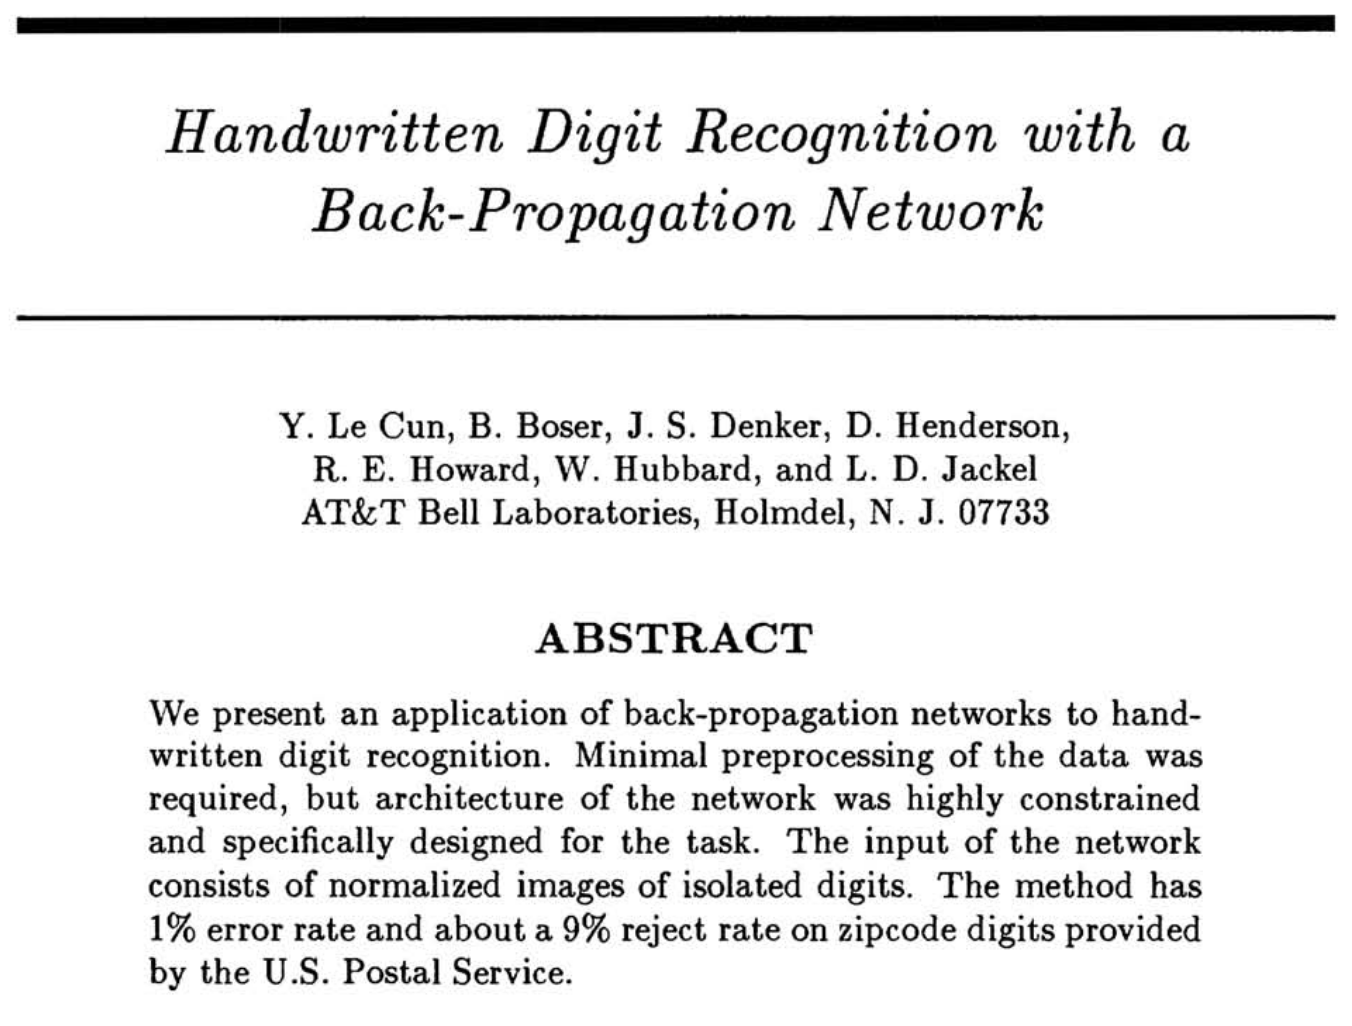
\includegraphics[width=0.4\paperwidth]{figure/lecun}}
    \subfigure{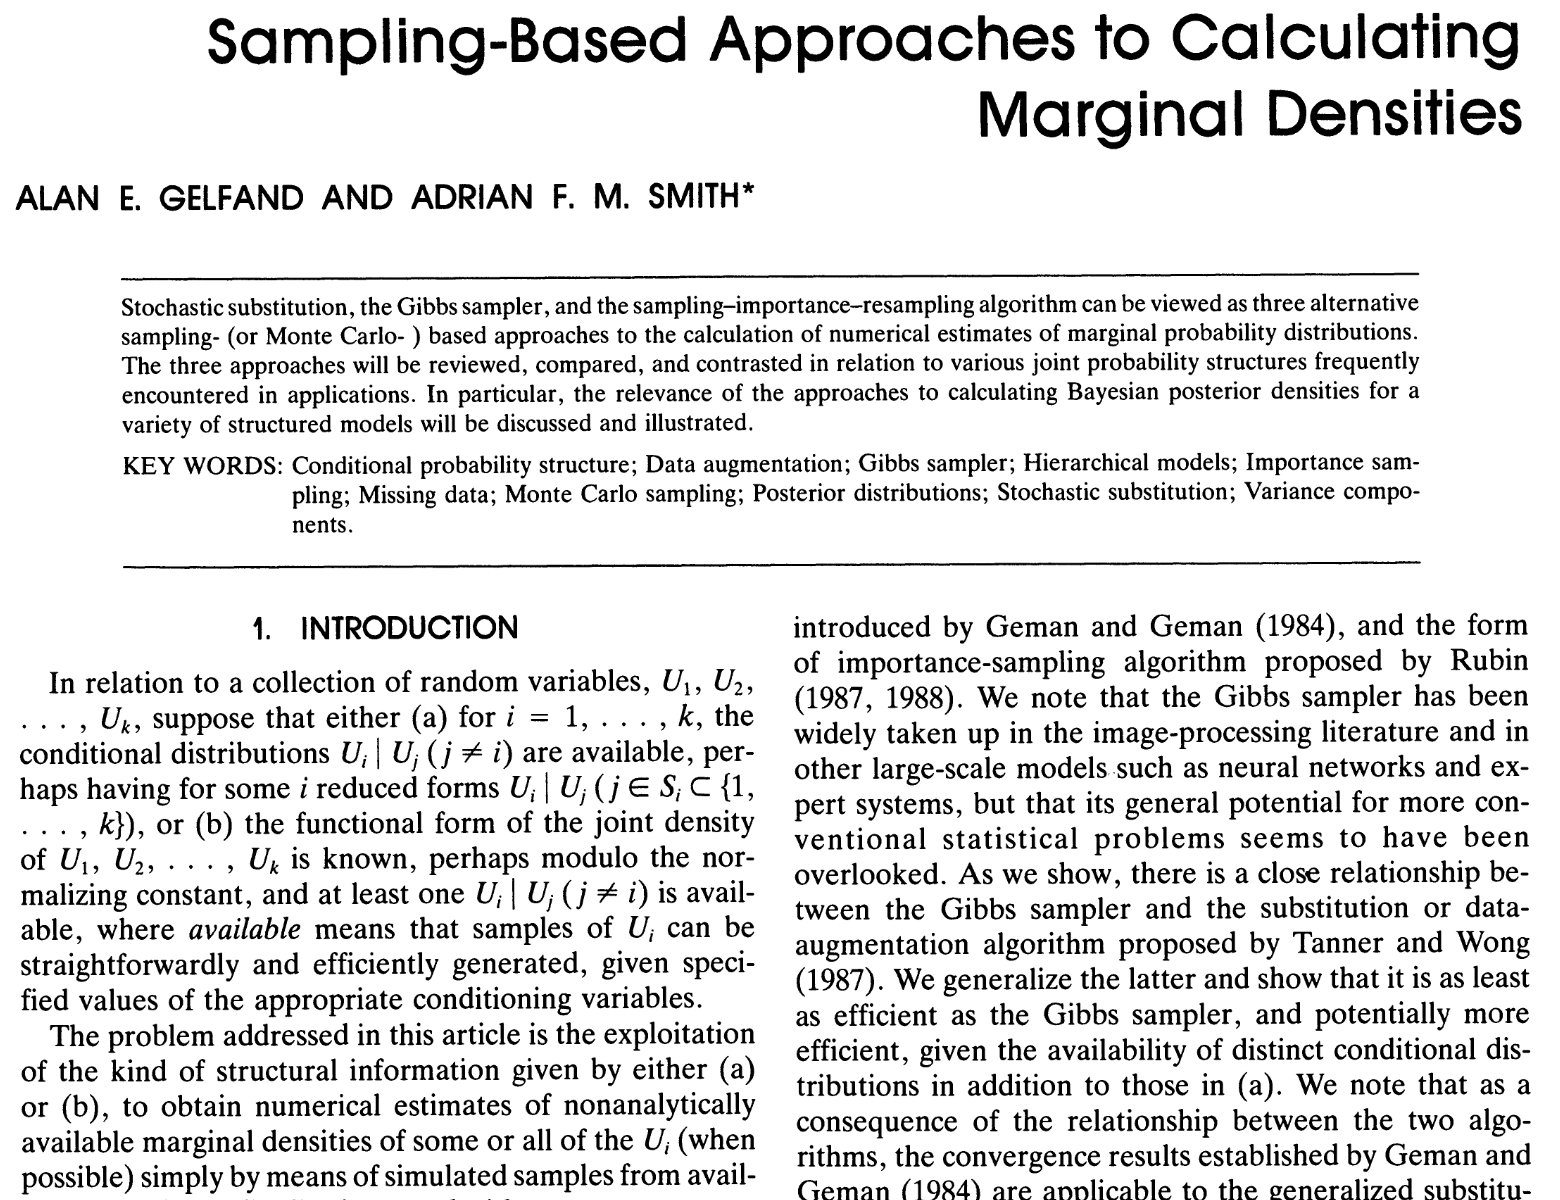
\includegraphics[width=0.4\paperwidth]{figure/gelfand}}
  \end{figure}
\end{frame}

\begin{frame}
  \frametitle{Reconciliation}
  \begin{itemize}
  \item We need both inference and prediction for systems that \textit{sense}
    and \textit{act} in the real world
    \begin{itemize}
    \item Need systems running in real time, interfacing with the world
    \item Probabilistic descriptions give us much more to base our decisions off of
    \item It would be nice if everything were automatic, or at least modular
    \end{itemize}
  \item Bayesian deep learning: modular feature learning with uncertainty
  \end{itemize}
  \begin{figure}
    \subfigure{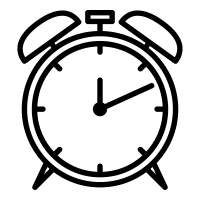
\includegraphics[width=0.2\paperwidth]{figure/clock}}
    \subfigure{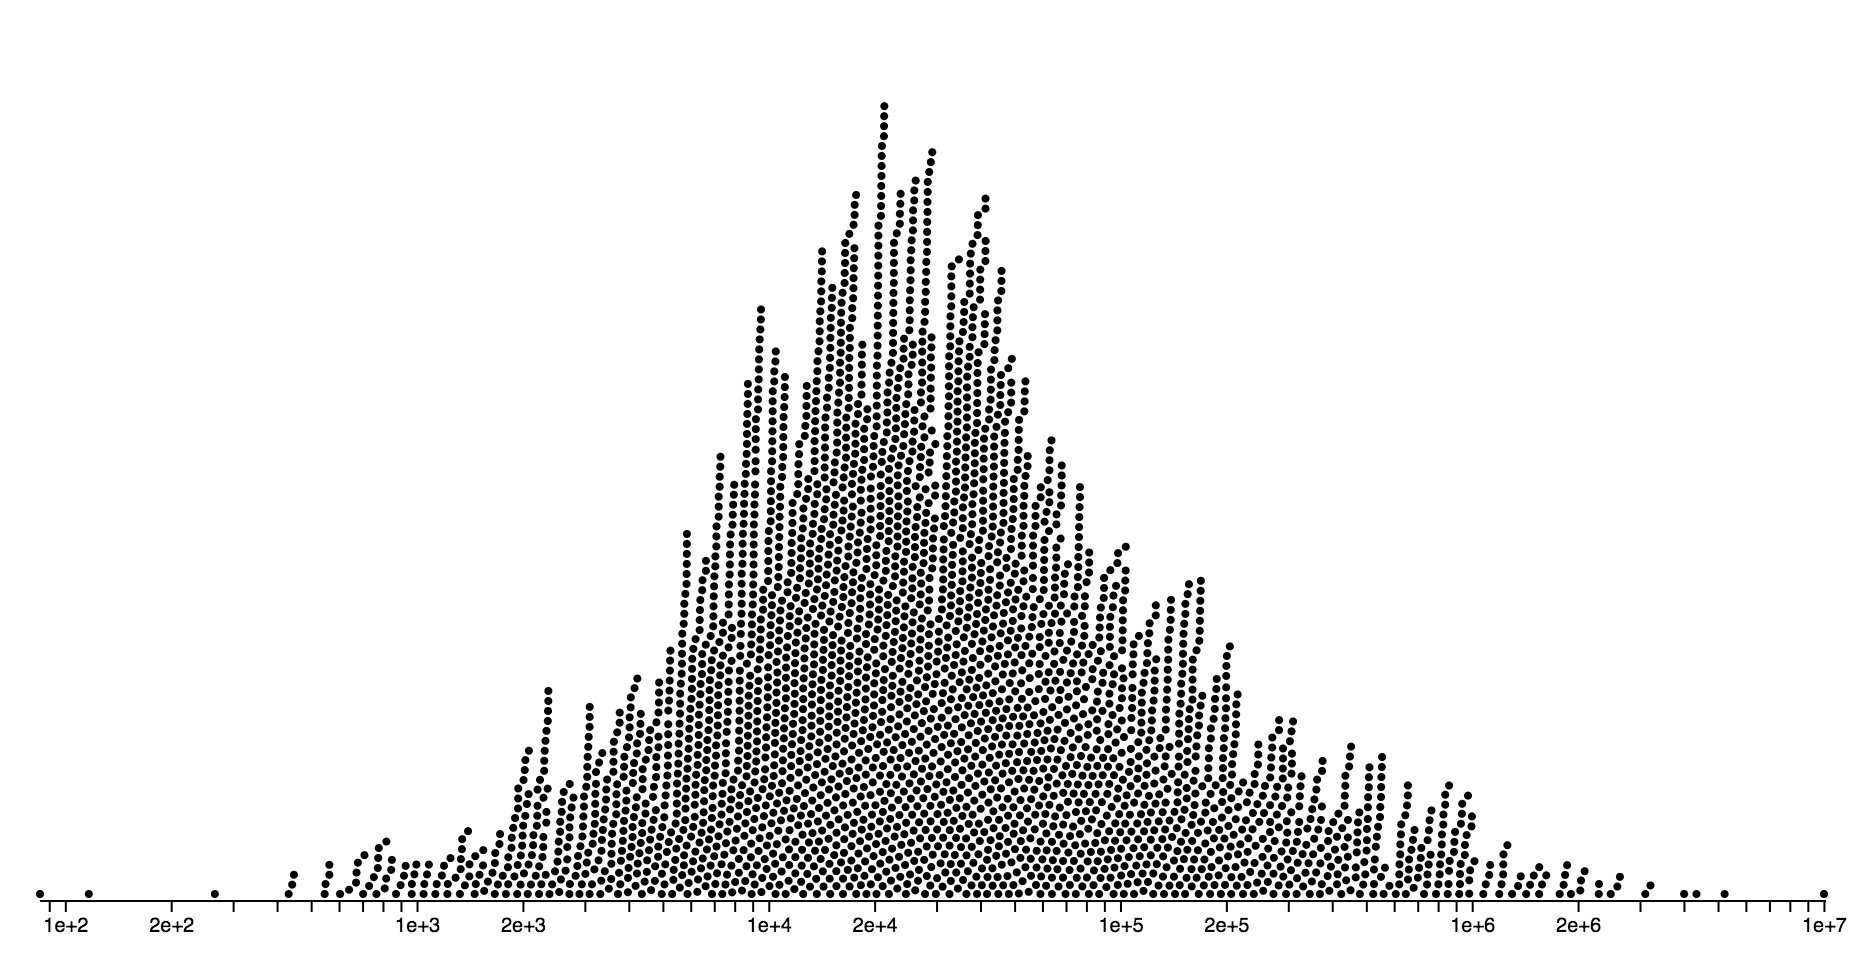
\includegraphics[width=0.3\paperwidth]{figure/beeswarm}}
    \subfigure{\includegraphics[width=0.15\paperwidth]{figure/robot.jpg}}
  \caption{We would like our modeling to be fast, probabilistic, and automatic.}
  \end{figure}
\end{frame}

\begin{frame}
  \frametitle{Machine Learning checklist}
  Questions to ask every algorithm you meet.
 \begin{itemize}
 \item What is the \textcolor{blue}{model class}?
 \item What is the \textcolor{green}{evaluation criterion}?
 \item What is the \textcolor{red}{search strategy}?
 \end{itemize}
\begin{figure}[ht]
  \centering
  \includegraphics[width=0.7\paperwidth]{figure/ml_overview}
  \caption{Each point in $\mathcal{F}$ represents a different function, which we
    evaluate using $\mathcal{L}$. We have to search through $\mathcal{F}$,
    represented by the red dashed line. \label{fig:ml_overview} }
\end{figure}
\end{frame}

\begin{frame}
  \frametitle{In Bayesian Deep Learning}
  Questions to ask every algorithm you meet.
 \begin{itemize}
 \item What is the \textcolor{blue}{model class}?
   \begin{itemize}
   \item Gaussian process?
   \item Mixture of multinomials?
   \item Gaussian with neural network $\mu_{\theta}$?
   \end{itemize}
 \item What is the \textcolor{green}{evaluation criterion}?
   \begin{itemize}
   \item Evidence
   \item Evidence Lower Bound
   \item Hold-out Log Likelihood
   \end{itemize}
 \item What is the \textcolor{red}{search strategy}?
   \begin{itemize}
   \item Variational Inference
   \item MCMC
   \item Expectation Propagation
   \end{itemize}
 \end{itemize}
\begin{figure}[ht]
  \centering
  \includegraphics[width=0.3\paperwidth]{figure/ml_overview}
  \caption{Each point in $\mathcal{F}$ represents a different function, which we
    evaluate using $\mathcal{L}$. We have to search through $\mathcal{F}$,
    represented by the red dashed line. \label{fig:ml_overview} }
\end{figure}
\end{frame}

\begin{frame}
  \frametitle{Classical Bayes}
  \begin{itemize}
  \item Bayes' Rule,
    \begin{align*}
      p\left(\theta \vert x\right) &= \frac{p\left(x \vert \theta\right)p\left(\theta\right)}{p\left(x\right)}
    \end{align*}
  \item Adapt your belief about $\theta$ after seeing $x$
  \item Specify likelihood $p\left(x \vert \theta\right)$ and prior $p\left(\theta\right)$
  \end{itemize}
\end{frame}

\begin{frame}
  \frametitle{Example: Beta-Binomial}
  \begin{itemize}
  \item Task: Identify potential bias in a coin
  \item Model specification,
    \begin{itemize}
    \item Prior: $p \sim \Bet\left(a_0, b_0\right)$
    \item Likelihood: $x \vert p \sim \Bin\left(n, p\right)$
    \end{itemize}
  \item Posterior is still a beta
  \end{itemize}
\begin{figure}[ht]
  \centering
  \includegraphics[width=0.6\paperwidth]{figure/betabinomial_video.png}
  \caption{After seeing more and more coin flips, the posterior becomes more
    sure that the underlying probability is around 0.2. \label{fig:betabinomial}
  }
\end{figure}
\end{frame}

\begin{frame}
  \frametitle{Beta-Binomial in Code}
  \begin{itemize}
  \item We can avoid doing any math by using the \texttt{pyro} package
  \item This is good practice for when it's impossible to do that math
  \item Hinges on the notion of a guide function
  \end{itemize}
  \begin{figure}[ht]
    \centering
    \includegraphics[width=0.7\paperwidth]{figure/pyro_model}
    \caption{Example implementation of beta-binomial model in a probabilistic
      programming language. \label{fig:pyro_model} }
  \end{figure}
\end{frame}

\begin{frame}
  \frametitle{Beta-Binomial in Code}
  \begin{itemize}
  \item We can avoid doing any math by using the \texttt{pyro} package
  \item This is good practice for when it's impossible to do that math
  \item Hinges on the notion of a guide function
  \end{itemize}
  \begin{figure}[ht]
    \centering
    \includegraphics[width=0.7\paperwidth]{figure/pyro_inference}
    \caption{Example implementation of beta-binomial inference in a
      probabilistic programming language. \label{fig:pyro_inference} }
\end{figure}
\end{frame}

\section{Latent Variable Models}
\label{sec:latent_variable_models}
\begin{frame}
  \frametitle{Mixture Models}
  \begin{itemize}
  \item Sometimes, critical parts of data generating mechanisms are unobserved
    \item Need posterior inference over both mixture parameters $\mu_k,
      \Sigma_k$ as well as assignments $z_i$
  \end{itemize}
  \begin{align*}
    \mu_{k} &\sim \Gsn\left(0, \Sigma_{0}\right) \\
    z_i &\sim \Cat\left(z_i \vert \pi\right) \\
    x_i \vert z_i = k &\sim \Gsn\left(x_i \vert \mu_{k}, \Sigma_k\right)
  \end{align*}
\begin{figure}[ht]
  \centering
  \includegraphics[width=0.35\paperwidth]{figure/gmm_1}
  \caption{We've drawn three gaussian densities from the overall prior, and mark
    an \texttt{X} at the first sample, along with its (in reality unobserved)
    class membership $z_i$. \label{fig:gmm_1} }
\end{figure}
\end{frame}

\label{sec:latent_variable_models}
\begin{frame}
  \frametitle{Mixture Models}
  \begin{itemize}
  \item Sometimes, critical parts of data generating mechanisms are unobserved
    \item Need posterior inference over both mixture parameters $\mu_k,
      \Sigma_k$ as well as assignments $z_i$
  \end{itemize}
  \begin{align*}
    \mu_{k} &\sim \Gsn\left(0, \Sigma_{0}\right) \\
    z_i &\sim \Cat\left(z_i \vert \pi\right) \\
    x_i \vert z_i = k &\sim \Gsn\left(x_i \vert \mu_{k}, \Sigma_k\right)
  \end{align*}
\begin{figure}[ht]
  \centering
  \includegraphics[width=0.35\paperwidth]{figure/gmm_2}
  \caption{Draw another point from the same cluster.
    \label{fig:gmm_2} }
\end{figure}
\end{frame}

\label{sec:latent_variable_models}
\begin{frame}
  \frametitle{Mixture Models}
  \begin{itemize}
  \item Sometimes, critical parts of data generating mechanisms are unobserved
    \item Need posterior inference over both mixture parameters $\mu_k,
      \Sigma_k$ as well as assignments $z_i$
  \end{itemize}
  \begin{align*}
    \mu_{k} &\sim \Gsn\left(0, \Sigma_{0}\right) \\
    z_i &\sim \Cat\left(z_i \vert \pi\right) \\
    x_i \vert z_i = k &\sim \Gsn\left(x_i \vert \mu_{k}, \Sigma_k\right)
  \end{align*}
\begin{figure}[ht]
  \centering
  \includegraphics[width=0.4\paperwidth]{figure/gmm_3}
  \caption{First point from a new cluster. \label{fig:gmm_3}}
\end{figure}
\end{frame}

\label{sec:latent_variable_models}
\begin{frame}
  \frametitle{Mixture Models}
  \begin{itemize}
  \item Sometimes, critical parts of data generating mechanisms are unobserved
    \item Need posterior inference over both mixture parameters $\mu_k,
      \Sigma_k$ as well as assignments $z_i$
  \end{itemize}
  \begin{align*}
    \mu_{k} &\sim \Gsn\left(0, \Sigma_{0}\right) \\
    z_i &\sim \Cat\left(z_i \vert \pi\right) \\
    x_i \vert z_i = k &\sim \Gsn\left(x_i \vert \mu_{k}, \Sigma_k\right)
  \end{align*}
\begin{figure}[ht]
  \centering
  \includegraphics[width=0.4\paperwidth]{figure/gmm_4}
  \caption{Continue in this way until you have all $n$ points. \label{fig:gmm_4}}
\end{figure}
\end{frame}

\begin{frame}
  \frametitle{Other Examples}
  \begin{itemize}
  \item Many widely-used models depend on being able to work with latent variables,
    \begin{itemize}
    \item Exponential Family PCA
    \item Hidden Markov Models
    \item Latent Dirichlet Allocation
    \end{itemize}
  \item Latent variables $z_i$ transform simple distributions (Gaussians) into
    complex ones (mixture of Gaussians)
  \item In general, mechanism is
    \begin{align*}
      \theta &\sim p_{\eta}\left(\theta\right) &\text{(prior on parameters)} \\
      z_{i} &\sim p_{\varphi}\left(z_{i}\right) &\text{(prior on latents)} \\
      x_{i} \vert z_{i}, \theta &\sim p_{\theta}\left(x_{i} \vert z_{i} \right) &\text{(likelihood)}
    \end{align*}
  \end{itemize}
  \begin{figure}[ht]
    \centering
    \includegraphics[width=0.2\paperwidth]{figure/mohamed_latent_variable}
    \caption{General form of a latent variable model, as given in
      \citep{mohamed2011generalised}. Replace our $z_i$'s with
      $v_n$'s. \label{fig:mohamed_latent_variable} }
  \end{figure}
\end{frame}

\begin{frame}
  \frametitle{Mixture of Gaussians: Complete Data Likelihood}
  If we know the mixture assignments $z_i$ for each sample, we could write out
  the likelihood very explicitly.
  \begin{align*}
\log p\left(x, z\right) &= \log \left[\prod_{i = 1}^{n} \prod_{k = 1}^{K} \left(p_{k}\Gsn\left(x_i \vert \mu_k, \Sigma_k\right)^{\indic{z_i = k}}\right)\right] \\
&= \sum_{i = 1}^{n} \sum_{k = 1}^{K} \indic{z_i = k} \left[\log p_{k} + \log \Gsn\left(x_i \vert \mu_k, \Sigma_k\right)\right] \\
&= \sum_{i = 1}^{n} \sum_{k = 1}^{K} \indic{z_i = k} \left[\log p_{k} -\frac{D}{2}\log\left(2\pi\right) - \frac{1}{2}\log \left|\Sigma_k\right| -  \\ &\qquad\frac{1}{2} \left(x_i - \mu_k\right)^{T}\Sigma^{-1}_{k} \left(x_i - \mu_k)\right]
  \end{align*}
\end{frame}

\begin{frame}
  \frametitle{Marginalizing $z$}
  \begin{itemize}
  \item How can we fit $\theta$ if we don't know the particular configuration of
    $z$?
  \item Way too many configurations to actual do this sum
  \end{itemize}
  \begin{align*}
    \log p_{\theta}\left(x\right) &= \log \sum_{z} p_{\theta}\left(x, z\right)
  \end{align*}
\end{frame}

\begin{frame}
  \frametitle{Evidence Lower Bound}
  \begin{itemize}
  \item It's counterintuitive, but one problem-solving strategy is to
    deliberately introduce complexity
  \item Complexity $\rightarrow$ more degrees of freedom
  \end{itemize}
\end{frame}

\begin{frame}
  \frametitle{Variational $q$}
  \begin{itemize}
  \item Consider some $q\left(z \vert x\right) \in \mathcal{Q}$, some large
    family of tractable densities
  \item Use age-old the ``multiply and divide by 1'' trick
  \end{itemize}
  \begin{align*}
    \log p_{\theta}\left(x\right) &= \Esubarg{q}{\log p_{\theta}\left(x\right)} \\
    &= \Esubarg{q}{\log \frac{p_{\theta}\left(x, z\right)}{p_{\theta}\left(z \vert x\right)}} \\
    &= \Esubarg{q}{\log \frac{p_{\theta}\left(x, z\right)}{q\left(z \vert x\right)} \frac{q\left(z \vert x\right)}{p_{\theta}\left(z \vert x\right)}} \\
    &= \Esubarg{q}{\log p_{\theta}\left(x \vert z\right)} - D_{KL}\left(q\left(z \vert x\right) \vert \vert p\left(z\right)\right) + D_{KL}\left(q\left(z \vert x\right) \vert \vert p_{\theta}\left(z \vert x\right)\right)
  \end{align*}
\end{frame}

\begin{frame}
  \frametitle{Studying the bound}
  \begin{align*}
    \log p_{\theta}\left(x\right) &= \textcolor{purple}{\Esubarg{q}{\log p_{\theta}\left(x \vert z\right)}} - \textcolor{blue}{D_{KL}\left(q\left(z \vert x\right) \vert \vert p\left(z\right)\right)} + \textcolor{orange}{D_{KL}\left(q\left(z \vert x\right) \vert \vert p_{\theta}\left(z \vert x\right)\right)} \\
     &\geq \textcolor{purple}{\Esubarg{q}{\log p_{\theta}\left(x \vert z\right)}} - \textcolor{blue}{D_{KL}\left(q\left(z \vert x\right) \vert \vert p_{\theta}\left(z\right)\right)}
  \end{align*}
  \begin{itemize}
  \item \textcolor{purple}{Reconstruction error}: How plausible is the observed
    $x$, averaging over assignments $z$, and considering the current likelihood
    estimate?
  \item \textcolor{blue}{Approximation complexity}: How far is the approximating
    $q\left(z \vert x\right)$ from the prior?
  \item \textcolor{orange}{Approximation quality}: How different is the
    posterior approximation $p\left(z \vert x\right)$
    from the actual posterior?
    \begin{itemize}
    \item $D_{KL} \geq 0$ for any pair of probabilities
    \item Hard to compute, so just drop and turn into an inequality
    \end{itemize}
  \end{itemize}
\end{frame}

\begin{frame}
  \frametitle{Variational Expectation Maximization (EM)}
  \begin{itemize}
  \item We now have a strategy for optimizing $\theta$'s
  \item Alternately update $\theta$ and $q\left(z \vert x\right)$ to maximize
    the ELBO
    \begin{itemize}
    \item E-Step: Find a distribution $q\left(z \vert x\right)$ over
      configurations $z$ that is most plausible with the current guess at
      $\theta$
    \item M-Step: Find a set of parameters $\theta$ that is most plausible with
      the current distribution over configurations $z$
    \end{itemize}
  \item Hope is that this also increases $p_{\theta}\left(x\right)$
  \end{itemize}
\end{frame}

\section{Variational Inference}
\label{sec:introduction}

\begin{frame}
  \frametitle{The Variational Idea}
  \begin{itemize}
  \item Transform integration problem into an optimization one
  \item Some families $\mathcal{Q}$ are easier to optimize over than others
  \end{itemize}
\begin{figure}[ht]
  \centering
  \includegraphics[width=0.45\paperwidth]{figure/variational_idea_1}
  \caption{The hope is to find a density $q^{\ast} \in \mathcal{Q}$ that's
    relatively close to the true posterior. \label{fig:variational_idea_1} }
\end{figure}
\end{frame}

\begin{frame}
  \frametitle{The Variational Idea}
  \begin{itemize}
  \item Transform integration problem into an optimization one
  \item Some families $\mathcal{Q}$ are easier to optimize over than others
  \end{itemize}
\begin{figure}[ht]
  \centering
  \includegraphics[width=0.5\paperwidth]{figure/variational_idea_2}
  \caption{Some families might be much easier to optimize over than others.
    \label{fig:variational_idea_1} }
\end{figure}
\end{frame}

\begin{frame}
  \frametitle{Doing Variational Inference}
  To practically implement this idea need to determine
  \begin{itemize}
  \item What densities $\mathcal{Q}$ can we actually work with?
  \item How are we going to measure the quality of an approximation?
  \end{itemize}
\end{frame}

\begin{frame}
  \frametitle{Doing Variational Inference}
  To practically implement this idea need to determine
  \begin{itemize}
  \item What densities $\mathcal{Q}$ can we actually work with?
    \begin{itemize}
    \item Mean-Field, Structured Mean-Field approximations, or even implicit densities
    \end{itemize}
  \item How are we going to measure the quality of an approximation?
    \begin{itemize}
    \item ELBO, $f$-divergences, Wasserstein distance, ...
    \end{itemize}
  \end{itemize}
\end{frame}

\begin{frame}
  \frametitle{Doing Variational Inference}
  To practically implement this idea need to determine
  \begin{itemize}
  \item What densities $\mathcal{Q}$ can we actually work with?
    \begin{itemize}
    \item \textbf{Mean-Field}, Structured Mean-Field approximations, or even implicit densities
    \end{itemize}
  \item How are we going to measure the quality of an approximation?
    \begin{itemize}
    \item \textbf{ELBO}, $f$-divergences, Wasserstein distance, ...
    \end{itemize}
  \end{itemize}
\end{frame}

\begin{frame}
  \frametitle{Mean-Field Approximation}
  Consider a family where all the variables factor
  \begin{align*}
    q\left(z_1, \dots, z_n\right) = \prod_{i = 1}^{n} q_{i}\left(z_i\right)
  \end{align*}
  (notice that we drop conditioning on $x_i$, this is actually more general than
  before)
\begin{figure}[ht]
  \centering
  \begin{subfigure}
    \includegraphics[width=0.2\paperwidth]{figure/variational_multidimensional_q}
  \end{subfigure}
  \begin{subfigure}
    \includegraphics[width=0.2\paperwidth]{figure/variational_univariate_q}
  \end{subfigure}
  \caption{Instead of trying to model the joint relationships across all the
    latent variables, we will concern ourselves with one coordinate at a
    time. \label{fig:variational_multidimensional_q}}
\end{figure}
\end{frame}

\begin{frame}
  \frametitle{Mean-Field Approximation}
  Consider a family where all the variables factor
  \begin{align*}
    q\left(z_1, \dots, z_n\right) = \prod_{i = 1}^{n} q_{i}\left(z_i\right)
  \end{align*}
  (notice that we drop conditioning on $x_i$, this is actually more general than
  before)
\begin{figure}[ht]
  \centering
  \begin{subfigure}
    \includegraphics[width=0.2\paperwidth]{figure/variational_multidimensional_q}
  \end{subfigure}
  \begin{subfigure}
    \includegraphics[width=0.2\paperwidth]{figure/variational_product_q}
  \end{subfigure}
  \caption{A consequence of using the product is that we can't model complex correlations between coordinates (everything has to be axis-aligned).
    \label{fig:variational_product_q}}
\end{figure}
\end{frame}

\begin{frame}
  \frametitle{Optimization}
  \begin{itemize}
  \item Fixing all but the $i^{th}$ coordinate's distribution, can find how to
    optimize ELBO directly
  \end{itemize}
  \begin{align*}
q_i\left(z_i\right) \propto \exp{\Esubarg{q_{-i}}{\log p\left(x, z_i, z_{-i}\right)}}
  \end{align*}
\end{frame}

%% Maybe put some examples of this update here
%% mention that this is a lot of algebra, every time you want a model

\begin{frame}
  The proof of this fact is only a few lines (not at all obvious though)
  \begin{align*}
    \log p\left(x\right) &\geq
    \Esubarg{q}{\log p\left(x \vert z\right)} - D_{KL}\left( q\left(z\right) \vert\vert p\left(z\right)\right) \\
    &= \Esubarg{q}{\log p\left(x, z\right)} - \Esubarg{q}{\log q\left(z\right)}\\
    &= \Esubarg{q_i}{\Esubarg{q_{-i \vert i}}{\log p\left(x, z_i, z_{-i}\right)}} - \sum \Esubarg{q_j}{\log q_j\left(z_j\right)} \\
    &\stackrel{c}{=} -D_{KL}\left(q_{i}\left(z_i\right) \vert \vert \exp{\Esubarg{q_{-i}}{p\left(x, z_i, z_{-i}\right)}}\right)
  \end{align*}
  Since KL is always $\geq 0$, can maximize this expression by setting it to zero
  (set $q_i$ to right hand side distribution)
\end{frame}

\section{Variational Autoencoders}

\begin{frame}
  \frametitle{A Calculated Tradeoff}
  \begin{itemize}
  \item It's nice that this approach works for arbitrary mean-field $\prod
    q_{i}\left(z_i\right)$
  \item But it's restrictive to have to compute
    \begin{align*}
      q_i\left(z_i\right) \propto \exp{\Esubarg{q_{-i}}{\log p\left(x, z_i, z_{-i}\right)}}
    \end{align*}
    in closed form (not to mention tedious)
    \begin{itemize}
    \item How could we have (say) $p\left(x \vert z\right) = \Gsn\left(x \vert
      \mu_{\theta}\left(z\right), \sigma^{2}_{\theta}\left(x\right)\right)$ for some
      complicated $\mu_{\theta}, \sigma^{2}_{\theta}$?
    \end{itemize}
  \end{itemize}
\begin{figure}[ht]
  \centering
  \includegraphics[width=0.6\paperwidth]{figure/vae_forwards}
  \caption{A flexible generative mechanism will let us map latent $z_i$'s into
    complex distributions in the $x_i$ space. This process is sometimes called
    ``decoding,'' because it takes an unobserved $z$ and transforms it into some
    $x$ living in the observation space. \label{fig:vae_forwards} }
\end{figure}

\end{frame}

\begin{frame}
  \frametitle{Inference Networks}
  \begin{itemize}
  \item Idea: Restrict family $\mathcal{Q}$ (hopefully not too much), and make
    optimization more automatic
  \item New approximating family: $q_{\varphi}\left(z \vert x\right) = \Gsn\left(z \vert
    \mu_{\varphi}\left(x\right), \sigma^{2}_{\varphi}\left(x\right) I\right)$
  \item Let $\mu_{\varphi}$ and $\sigma^{2}_{\varphi}$ be arbitrary nonlinear
    functions
    \begin{figure}
        \centering
        \includegraphics[width=0.45\paperwidth]{figure/vae_inference}
        \caption{Each $x_i$ is associated with it's own distribution in the
          $z_i$ space. The parameters of this distribution are determined by the
          inference network. This process is sometimes called ``encoding,''
          because it encodes an observed $x$ into a latent
          $z$. \label{fig:vae_inference} }
    \end{figure}
  \end{itemize}
\end{frame}

\begin{frame}
  \frametitle{Optimization}
\begin{itemize}
\item Instead of optimizing one coordinate at a time, optimize all at once
  through $\varphi$
\item Simulatneously optimize parameters $\theta$
\item Essentially variational EM, but where $q$ is a parameterized function of
  the $x_{i}$
\end{itemize}
\end{frame}

\begin{frame}
  \frametitle{Reparametrization Trick}
  \begin{itemize}
  \item Taking gradient step along
  \begin{align*}
    \nabla_{\varphi} \Esubarg{q}{\log p_{\theta}\left(x \vert z\right)}
  \end{align*}
  is complicated, because
  \begin{align*}
    \nabla_{\varphi} \Esubarg{q}{\log p_{\theta}\left(x \vert z\right)} &= \int \log p_{\theta}\left(x \vert z\right)
    \nabla_{\varphi}q_{\varphi}\left(z \vert x\right)dz
  \end{align*}
  is no longer an expectation over $q_{\varphi}$.
  \item Can't just sample, and can't do integral analytically.
  \end{itemize}
\end{frame}

\begin{frame}
  \frametitle{Reparametrization Trick}
  \begin{itemize}
  \item Sampling
  \begin{align*}
    z \vert x \sim q_{\varphi}\left(z \vert x\right)
  \end{align*}
  is sometimes the same as
  \begin{align*}
    \eps &\sim p_{0}\left(\eps\right) \\
    z \vert \eps, x &\equiv g_{\varphi}\left(x, \eps\right)
  \end{align*}
  for some deterministic $g_{\varphi}$
  \item Large family of densities $\rightarrow$ one density with large family of
    transformations
  \end{itemize}
\end{frame}

\begin{frame}
  \frametitle{Reparametrization Trick}
  Most common example, if you want to sample
  \begin{align*}
    z \vert x &\sim \Gsn\left(z \vert \mu_{\varphi}\left(x\right), \sigma_{\varphi}^{2}\left(x\right)\right)
  \end{align*}
  instead use
  \begin{align*}
    \eps &\sim \Gsn\left(0, I\right) \\
    z \vert x, \eps &\equiv \mu_{\varphi}\left(x\right) + \sigma_{\varphi}^{2}\left(x\right) \odot \eps
  \end{align*}
\begin{figure}[ht]
  \centering
  \includegraphics[width=0.25\paperwidth]{figure/reparameterization_geometry}
  \caption{Instead of working with multiple gaussian densities (purple and red
    gaussians), we work with one and transform it with different linear
    transformations. \label{fig:reparameterization_geometry} }
\end{figure}

\end{frame}

\begin{frame}
  \frametitle{Optimization after Reparameterization}
  \begin{itemize}
  \item Since $g_{\varphi}$ is deterministic, gradient can be easily
    approximated,
  \begin{align*}
    \nabla_{\varphi} \Esubarg{q_{\varphi}}{\log p_{\theta}\left(x \vert z\right)} &=
    \nabla_{\varphi} \Esubarg{p\left(\eps\right)}{\log p_{\theta}\left(x \vert g_{\varphi}\left(\eps\right)\right)} \\
    &= \Esubarg{p\left(\eps\right)}{\nabla_{\varphi} \log p_{\theta}\left(x \vert g_{\varphi}\left(\eps\right)\right)} \\
      &\approx \sum_{i} \nabla_{\varphi} \log_{\theta}p_{\theta}\left(x \vert g_{\varphi}\left(\eps_{i}\right)\right)
  \end{align*}
  after sampling lots of $\eps_{i} \sim p\left(\eps\right)$.
  \item Derivative of $D_{KL}$ term can usually be written in closed form
  \item We can optimize the ELBO!
  \end{itemize}
\end{frame}

\section{Applications}
\label{sec:applications}

\begin{frame}
  \frametitle{Latent Space \& Generation}
\begin{figure}[ht]
  \centering
  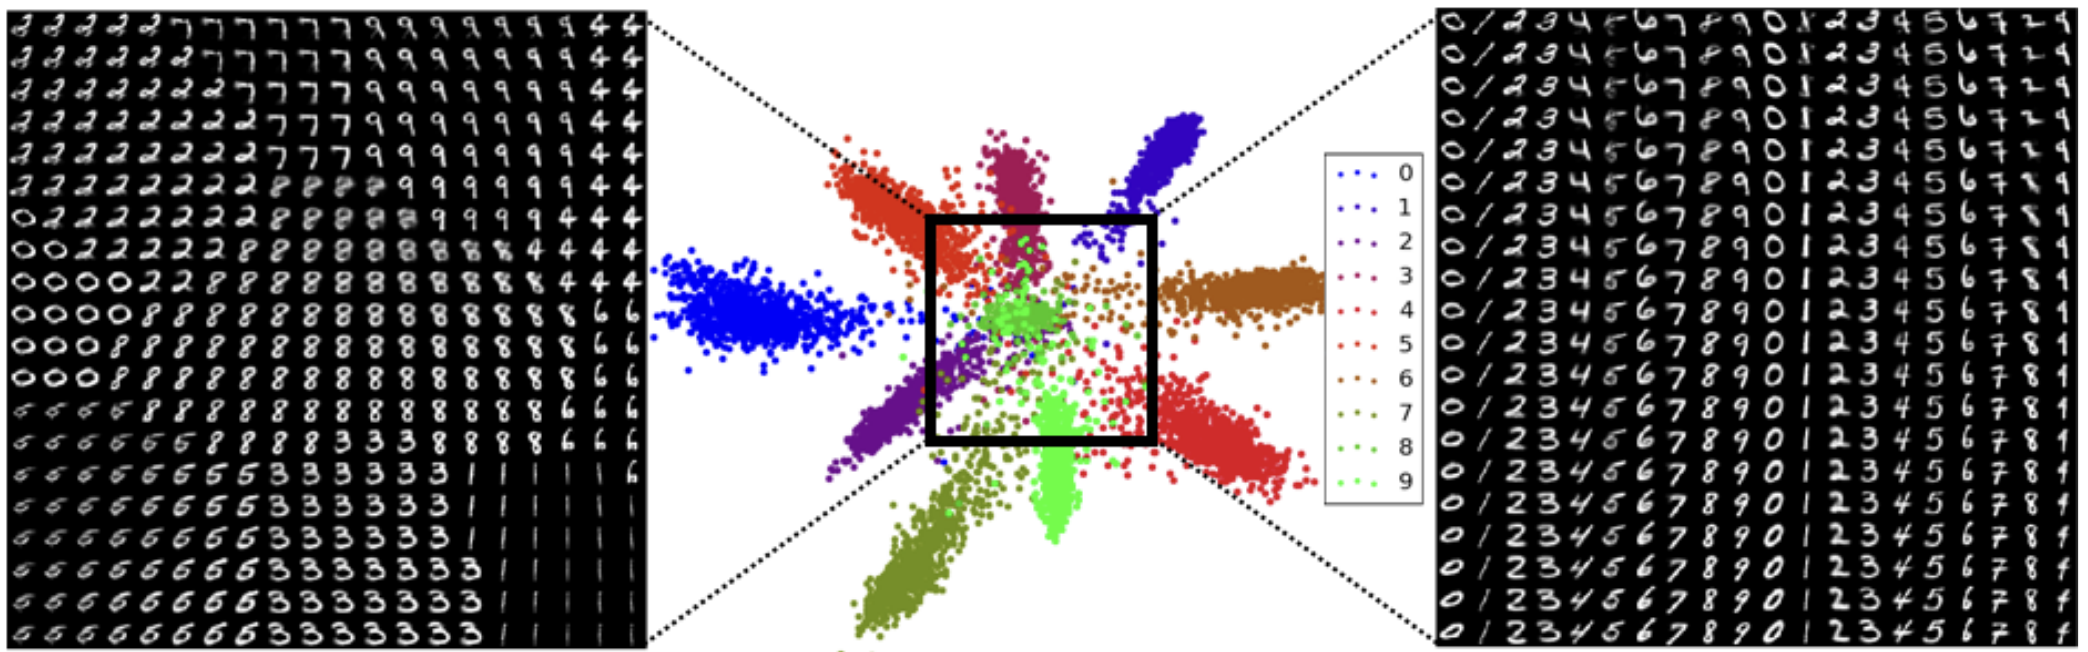
\includegraphics[width=0.8\paperwidth]{figure/vae_latent}
  \caption{The latent space (center) clearly distinguishes between different
    MNIST classes. From a given point in the latent space, we can generate many
    different images. \label{fig:vae_latent} }
\end{figure}
\end{frame}

\begin{frame}
  \frametitle{Drug Design \& Discovery}
\begin{figure}[ht]
  \centering
  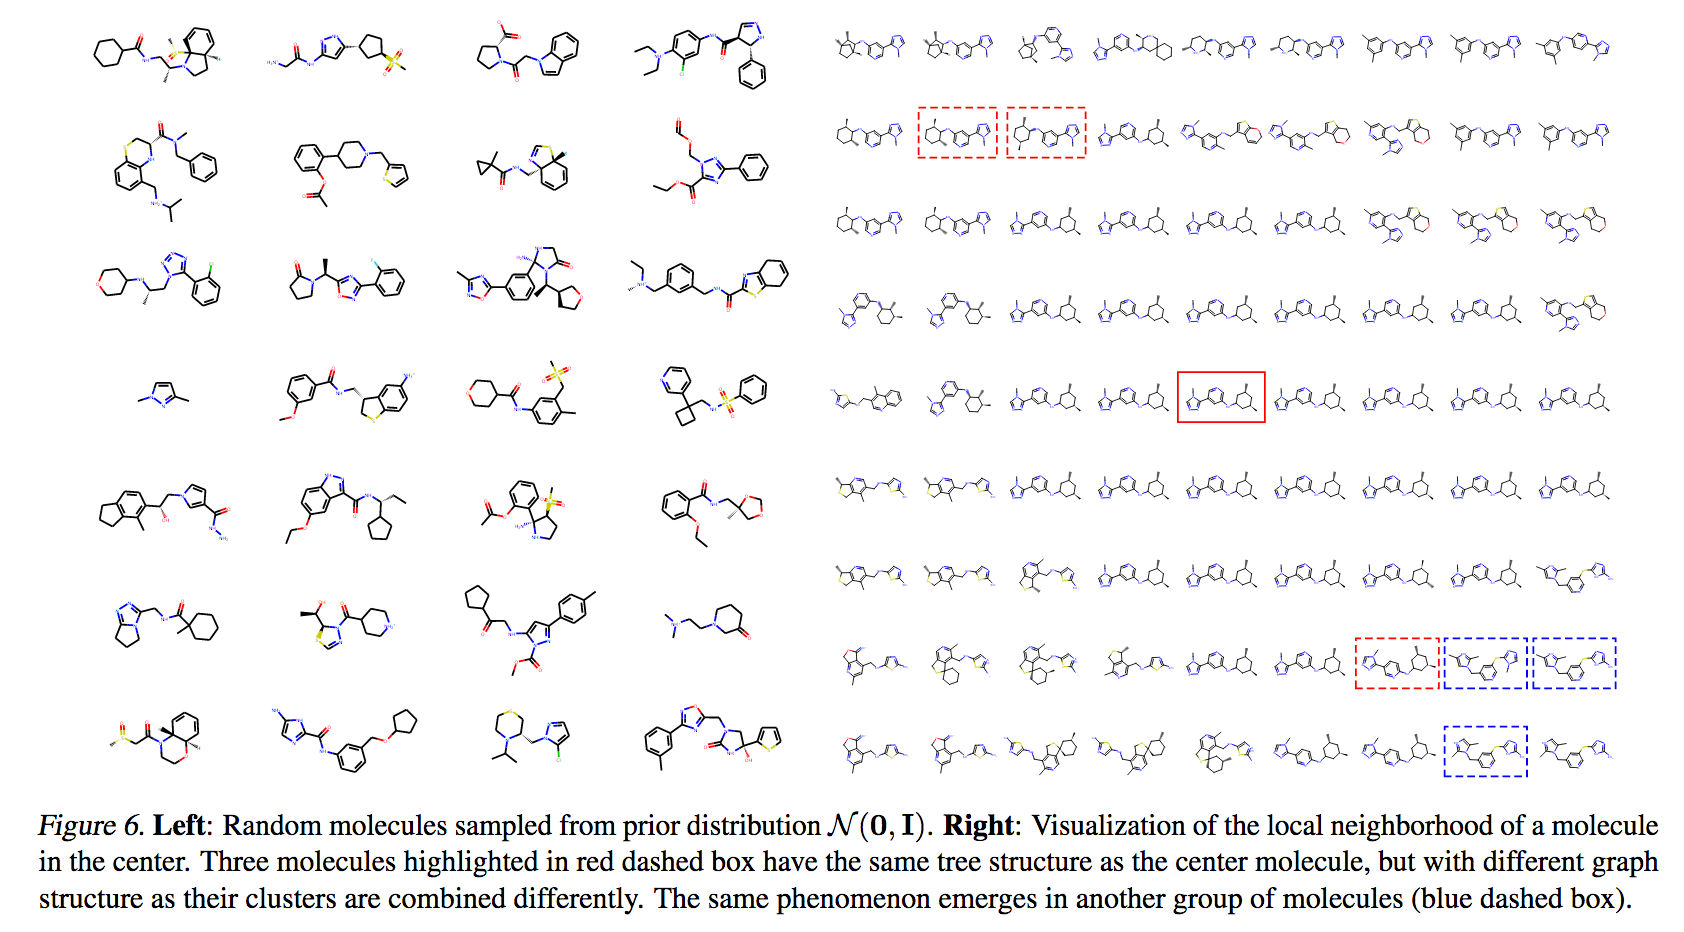
\includegraphics[width=0.6\paperwidth]{figure/vae_molecule}
  \caption{We can learn a latent space over molecules, and then sample molecules
    from different parts of the space. This gives a simple way of comparing
    molecular structures, which are otherwise complicated objects to try to
    compare. Image taken from \citep{jin2018junction}}
\end{figure}
\end{frame}

\begin{frame}
  \frametitle{Probabilistic Tumor Segmentation}
\begin{figure}[ht]
  \centering
  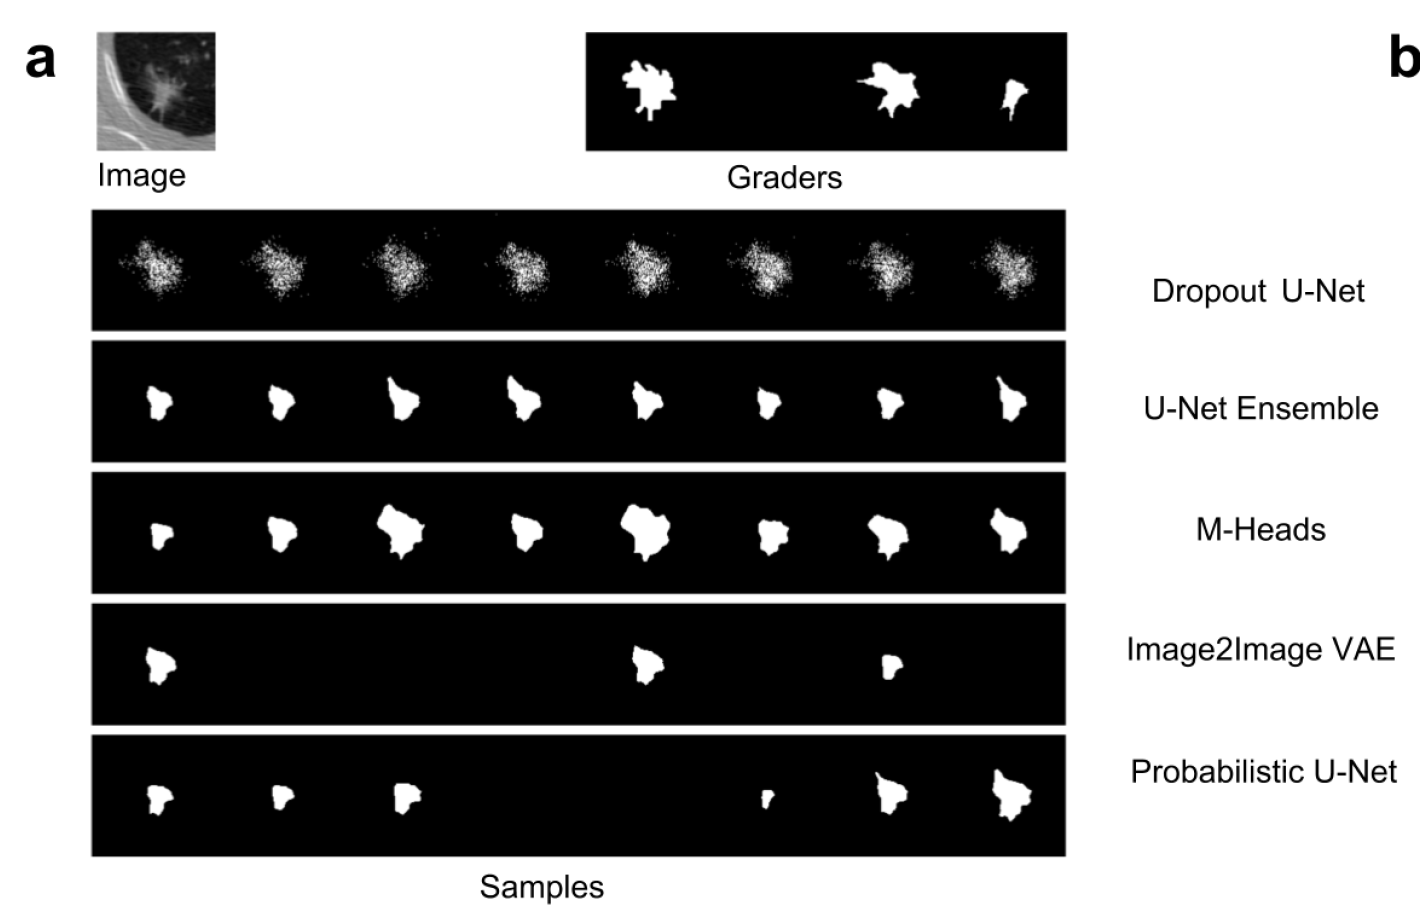
\includegraphics[width=0.6\paperwidth]{figure/vae_unet}
  \caption{A probabilistic model over tumor segmentations allows doctors to view
    several plausible views associated with a single X-ray
    image. Example taken from
    \citep{kohl2018probabilistic}. \label{fig:vae_unet} }
\end{figure}
\end{frame}

\begin{frame}
  \frametitle{Conditional Sample}
\begin{figure}[ht]
  \centering
  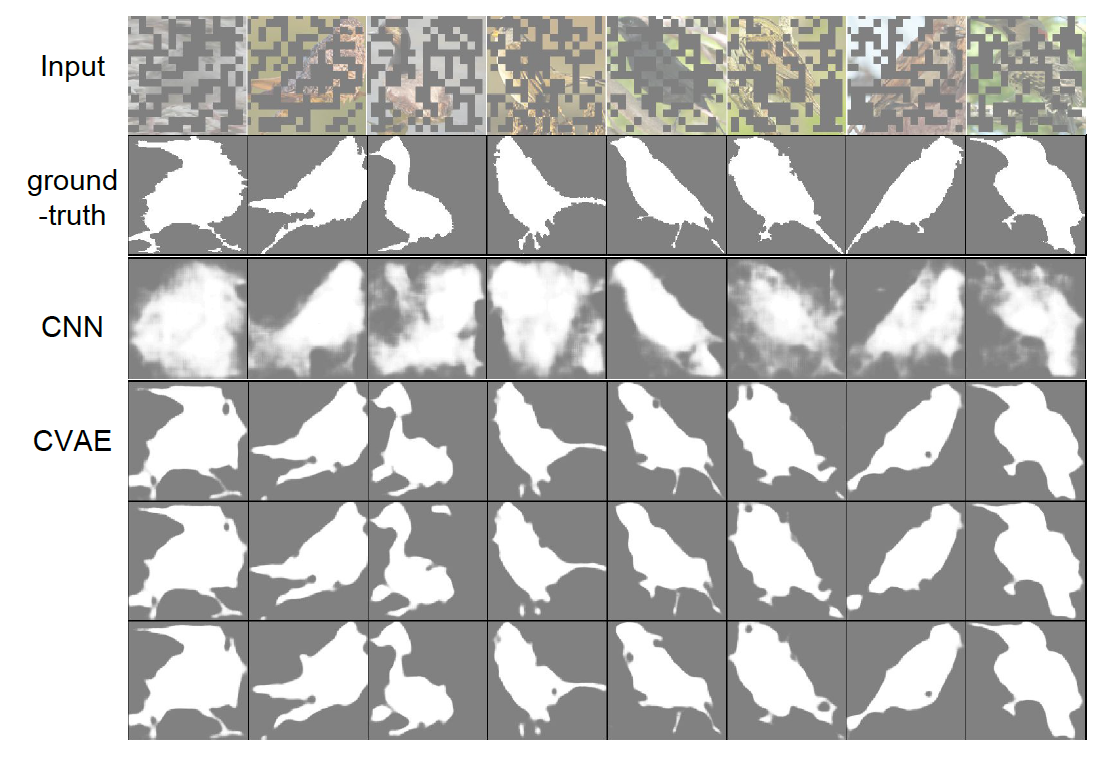
\includegraphics[width=0.6\paperwidth]{figure/vae_conditional}
  \caption{Since the VAE is a probabilistic model, we can condition on partial
    information. Here, a segmentation is conditioned on only partially observed
    input images. \label{fig:vae_conditional} }
\end{figure}
\end{frame}

\begin{frame}
  \frametitle{One-Shot Generalization}
  \begin{figure}[ht]
  \centering
  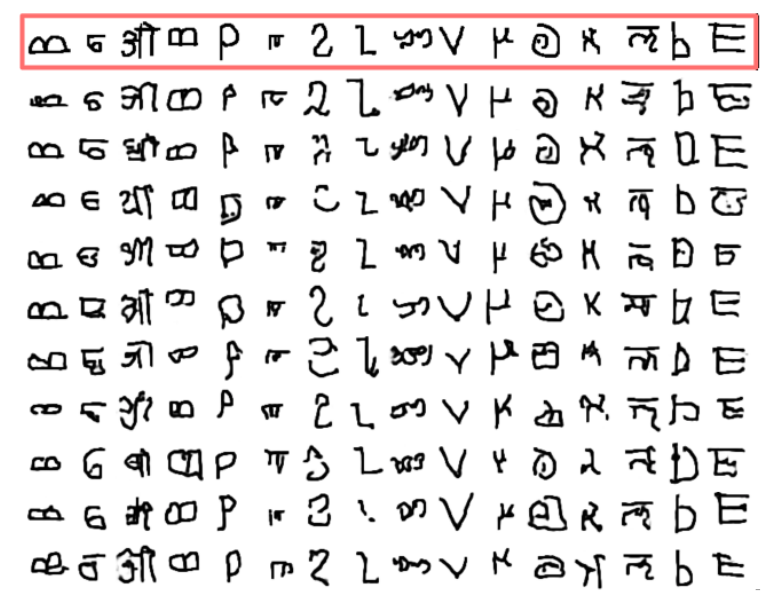
\includegraphics[width=0.5\paperwidth]{figure/vae_omniglot}
  \caption{Given only a few observations from one class, we can start to
    generate images that look like it, after encoding it properly. Example taken
    from \citep{rezende2016one}.}
\end{figure}
\end{frame}

\begin{frame}
  \frametitle{Conclusion}
  \begin{itemize}
  \item Latent variables are useful devices for introducing complexity
  \item To fit latent variable models, need to simultaneously optimize
    \begin{itemize}
    \item Configuration $z$'s consistent with observed data
    \item Global parameters $\theta$ generating data
    \end{itemize}
  \item Variational Autoencoders approximate full mean-field inference using an
    inference network with shared parameters
    \begin{itemize}
    \item Allows application to settings where forwards model is not amenable to
      analytical formulas
    \end{itemize}
  \end{itemize} 
\end{frame}

\end{document}
